\documentclass[
  bibliography=totoc,     % Literatur im Inhaltsverzeichnis
  captions=tableheading,  % Tabellenüberschriften
  titlepage=firstiscover, % Titelseite ist Deckblatt
]{scrartcl}

% Paket float verbessern
\usepackage{scrhack}

% Warnung, falls nochmal kompiliert werden muss
\usepackage[aux]{rerunfilecheck}

% unverzichtbare Mathe-Befehle
\usepackage{amsmath}
% viele Mathe-Symbole
\usepackage{amssymb}
% Erweiterungen für amsmath
\usepackage{mathtools}

% Fonteinstellungen
\usepackage{fontspec}
% Latin Modern Fonts werden automatisch geladen
% Alternativ:
%\setromanfont{Libertinus Serif}
%\setsansfont{Libertinus Sans}
%\setmonofont{Libertinus Mono}
\recalctypearea % Wenn man andere Schriftarten gesetzt hat,
% sollte man das Seiten-Layout neu berechnen lassen

% deutsche Spracheinstellungen
\usepackage{polyglossia}
\setmainlanguage{german}


\usepackage[
  math-style=ISO,    % ┐
  bold-style=ISO,    % │
  sans-style=italic, % │ ISO-Standard folgen
  nabla=upright,     % │
  partial=upright,   % ┘
  warnings-off={           % ┐
    mathtools-colon,       % │ unnötige Warnungen ausschalten
    mathtools-overbracket, % │
},                       % ┘
]{unicode-math}

% traditionelle Fonts für Mathematik
\setmathfont{Latin Modern Math}
% Alternativ:
%\setmathfont{Libertinus Math}

\setmathfont{XITS Math}[range={scr, bfscr}]
\setmathfont{XITS Math}[range={cal, bfcal}, StylisticSet=1]

% Zahlen und Einheiten
\usepackage[
locale=DE,                   % deutsche Einstellungen
separate-uncertainty=true,   % immer Fehler mit \pm
per-mode=symbol-or-fraction, % / in inline math, fraction in display math
]{siunitx}

% chemische Formeln
\usepackage[
version=4,
math-greek=default, % ┐ mit unicode-math zusammenarbeiten
text-greek=default, % ┘
]{mhchem}

% richtige Anführungszeichen
\usepackage[autostyle]{csquotes}

% schöne Brüche im Text
\usepackage{xfrac}

% Standardplatzierung für Floats einstellen
\usepackage{float}
\floatplacement{figure}{htbp}
\floatplacement{table}{htbp}

% Floats innerhalb einer Section halten
\usepackage[
section, % Floats innerhalb der Section halten
below,   % unterhalb der Section aber auf der selben Seite ist ok
]{placeins}

% Seite drehen für breite Tabellen: landscape Umgebung
\usepackage{pdflscape}

% Captions schöner machen.
\usepackage[
  labelfont=bf,        % Tabelle x: Abbildung y: ist jetzt fett
  font=small,          % Schrift etwas kleiner als Dokument
  width=0.9\textwidth, % maximale Breite einer Caption schmaler
]{caption}
% subfigure, subtable, subref
\usepackage{subcaption}

% Grafiken können eingebunden werden
\usepackage{graphicx}
% größere Variation von Dateinamen möglich
\usepackage{grffile}

% schöne Tabellen
\usepackage{booktabs}

% Verbesserungen am Schriftbild
\usepackage{microtype}

% Literaturverzeichnis
\usepackage[style=alphabetic,]{biblatex}
% Quellendatenbank
\addbibresource{lit.bib}
\addbibresource{programme.bib}

% Hyperlinks im Dokument
\usepackage[
  unicode,        % Unicode in PDF-Attributen erlauben
  pdfusetitle,    % Titel, Autoren und Datum als PDF-Attribute
  pdfcreator={},  % ┐ PDF-Attribute säubern
  pdfproducer={}, % ┘
]{hyperref}
% erweiterte Bookmarks im PDF
\usepackage{bookmark}

% Trennung von Wörtern mit Strichen
\usepackage[shortcuts]{extdash}

\usepackage{pdflscape}

\title{V27: Der Zeeman-Effekt}
\author{
  Simon Schulte
  \texorpdfstring{
    \\
    \href{mailto:simon.schulte@udo.edu}{simon.schulte@udo.edu}
  }{}
  \texorpdfstring{\and}{, }
  Tim Sedlaczek
  \texorpdfstring{
    \\
    \href{mailto:tim.sedlaczek@udo.edu}{tim.sedlaczek@udo.edu}
  }{}
}
\publishers{TU Dortmund – Fakultät Physik}

\date{Durchführung: 11.07.2018\\
      Abgabe: 14.09.2018}


\begin{document}

\maketitle
\thispagestyle{empty}
\setcounter{page}{1}
\pagenumbering{arabic}
\section{Theorie}
Wenn Atome von einem Magnetfeld beeinflusst werden, tritt der Zeeman-Effekt auf.
Dadurch ändern sich die Energieniveaus des jeweiligen Atoms. \\
\\
Experimentell lässt sich die Verschiebung über die Aufspaltung und Polarisation
der durch die Atome emittierten Spektrallinien untersuchen. Über sogenannte
Auswahlregeln lassen sich in der Theorie Vorhersagen über die Energie und
Polarisation der emittierten Strahlung machen.
%
\subsection{Drehimpuls und magnetisches Moment eines Elektrons}
%
Jedes Hüllenelektron besitzt zwei Drehimpulse, den Bahndrehimpuls~$\vec{l}$ und
den Spin~$\vec{s}$. Die Lösungen der quantenmechanischen Eigenwertgleichungen
liefern für die Beträge der Drehimpulse:
%
\begin{align}
    \lvert\,\vec{l}\,\rvert&=\sqrt{l(l+1)}\,\hbar\quad\text{mit}\quad l=0,1,2,\ldots,n-1
    \shortintertext{und}
    \lvert\,\vec{s}\,\rvert&=\sqrt{s(s+1)}\,\hbar\quad\text{mit}\quad s=\frac{1}{2}.
\end{align}
%
Die Drehimpulse bedingen je ein magnetisches Moment. Der Bahndrehimpuls liefert
%
\begin{gather}
    \vec{\mu}_l=-\mu_{\mathup{B}}\sqrt{l(l+1)}\,\vec{l}_0
    \intertext{mit dem Bohrschen Magneton}
    \mu_{\mathup{B}}:=-\frac{e_0\hbar}{2m_0}.
\end{gather}
%
Der Spin liefert
%
\begin{equation}
    \vec{\mu}_s=-g_s\sqrt{s(s+1)}\,\vec{s}_0
\end{equation}
%
mit dem Landé-Faktor~$g_s$ des Elektrons, der etwa den Wert~$2$ hat.
Für den Zustand mit $s=\frac{1}{2}$ und $l=1$ ist $\vec{\mu}_s$ ungefähr
doppelt so groß wie $\vec{\mu}_l$. Der exakte Wert von $g_s$
ergibt sich aus der relativistischen Theorie des Elektrons nach Dirac.

\subsection{Wechselwirkungen der Drehimpulse und der magnetischen Momente}
%
Im Folgenden werden die Wechselwirkungen der Drehimpulse eines
Mehrelektronenatoms betrachtet. Die beiden Drehimpulse eines Elektrons
wechselwirken sowohl untereinander, als auch mit den Drehimpulsen anderer
Elektronen in der Hülle. Diese Überlagerung der Wechselwirkungen ist in der
Theorie schwer zu beschreiben. Daher werden 2 Fälle betrachtet. \\
\\
\noindent
\textbf{1. Fall:}
Bei Atomen mit niedriger Kernladungszahl ist die Wechselwirkung zwischen den
Bahndrehimpulsen verschiedener Elektronen so groß, dass sich diese zum
Gesamtbahndrehimpuls~$\vec{L}$ addieren, wobei
%
\begin{align}
    \lvert\,\vec{L}\,\rvert&=\sqrt{L(L+1)}\,\hbar\quad\text{mit}\quad L=0,1,2,\ldots
    \intertext{gilt. Gemäß der gebräuchlichen Notation in der Atomphysik werden die verschiedenen Werte von $L$ aufsteigend mit den Buchstaben $S,P,D,F,\ldots$ gekennzeichnet. Analog zu den Bahndrehimpulsen kombinieren sich auch die Spins der Elektronen additiv zum Gesamtspin~$\vec{S}$. Es gilt}
    \lvert\,\vec{S}\,\rvert&=\sqrt{S(S+1)}\,\hbar\quad\text{mit}\quad S=\frac{N}{2},\frac{N}{2}-1,\ldots,\frac{1}{2},0
\end{align}
%
wobei $N$ die Anzahl der Hüllenelektronen ist.
Auch dem Gesamtbahndrehimpuls~$\vec{L}$ und dem Gesamtspin~$\vec{S}$ wird mit
%
\begin{align}
    \lvert\,\vec{\mu}_L\,\rvert&=\mu_{\mathup{B}}\sqrt{L(L+1)}
    \shortintertext{und}
    \lvert\,\vec{\mu}_S\,\rvert&=g_S\mu_{\mathup{B}}\sqrt{S(S+1)}
\end{align}
%
ein magnetisches Moment zugeordnet.
Für nicht zu starke Magnetfelder ergibt sich ein Gesamtdrehimpuls
%
\begin{gather}
    \vec{J}=\vec{L}+\vec{S}
    \shortintertext{mit}
    \lvert\,\vec{J}\,\rvert=\sqrt{J(J+1)}
\end{gather}
%
wobei $J$ entweder ganz- oder halbzahlig sein kann.
Der obige Zusammenhang wird auch als $LS$-Kopplung oder
Russell-Saunders-Kopplung bezeichnet. $J$ wird üblicherweise als unterer Index
an den Symbolen $S,P,D,F,\ldots$ notiert. Oberer Index ist die Multiplizität $M=2S+1$. \\
\\
\noindent
\textbf{2. Fall:}
Bei schweren Atomen ist die Wechselwirkung zwischen Spin und Bahndrehimpuls
eines Elektrons groß gegenüber der Wechselwirkung der Bahndrehimpulse und Spins
verschiedener Elektronen untereinander. Es ergibt sich der Gesamtdrehimpuls
%
\begin{equation}
    \vec{j}_i=\vec{l}_i+\vec{s}_i
\end{equation}
%
je Einzelektron, sodass kein Gesamtdrehimpuls~$\vec{L}$ und Gesamtspin $\vec{S}$
mehr definiert sind. Die $\vec{j}_i$ addieren sich nun zum Gesamtdrehimpuls $\vec{J}$.
Diese Art der Wechselwirkung wird auch als $j$-$j$-Kopplung bezeichnet.
\noindent
Zwischen den genannten Grenzfällen existiert für mittlere Kernladungszahlen ein
fließender Übergang.
%
\subsection{Aufspaltung der Energieniveaus eines Atoms im homogenen Magnetfeld}
%
Das zu $\vec{J}$ gehörende magnetische Moment ergibt sich zu
%
\begin{equation}
    \vec{\mu}=\vec{\mu}_L+\vec{\mu}_S.
\end{equation}
%
$\vec{J}$ und $\vec{\mu}$ sind im Allgemeinen nicht parallel, doch der
Erwartungswert der zu $\vec{J}$ senkrechten Komponente verschwindet aufgrund
der präzedierenden Bewegung um die Magnetfeldrichtung im zeitlichen Mittel.
Aus der Quantenmechanik folgt
%
\begin{equation}
     \lvert\,\vec{\mu}_J\,\rvert=g_J\mu_{\mathup{B}}\sqrt{J(J+1)}
\end{equation}
%
mit dem Landé-Faktor
%
\begin{equation}
    g_J:=\frac{3J(J+1)+S(S+1)-L(L+1)}{2J(J+1)}.
    \label{eq:g_J}
\end{equation}
%
Ein weiteres Resultat der Quantenmechanik ist die Richtungsquantelung im
homogenen Magnetfeld. Es gilt:
%
\begin{equation}
    \mu_{J_z}=-mg_J\mu_{\mathup{B}}
\end{equation}
%
mit der Orientierungsquantenzahl $m\in\{-J,-J+1,\ldots,J-1,J\}$.
Daraus folgen $2J+1$ Einstellmöglichkeiten für ein magnetisches Moment in einem
äußeren Magnetfeld. Für die Energie, die ein Moment $\vec{\mu}$ im Magnetfeld
erhält, ergibt sich:
%
\begin{equation}
    E_{\mathup{mag}}=-\vec{\mu}\vec{B}=mg_J\mu_{\mathup{B}}B.
    \label{eq:E_mag}
\end{equation}
%
Das Energieniveau $E_0$ im feldfreien Raum spaltet bei $B\neq0$ in $2J+1$
äquidistante Niveaus auf. Beispielhaft ist dies in Abbildung
\ref{fig:aufspaltung} für ein Atom mit $J=2$ skizziert. Die Aufspaltung
ermöglicht neue Übergänge zwischen Energieniveaus und somit neue Spektrallinien.
Dieser Effekt wird als Zeeman-Effekt bezeichnet.
%
\begin{figure}
    \centering
    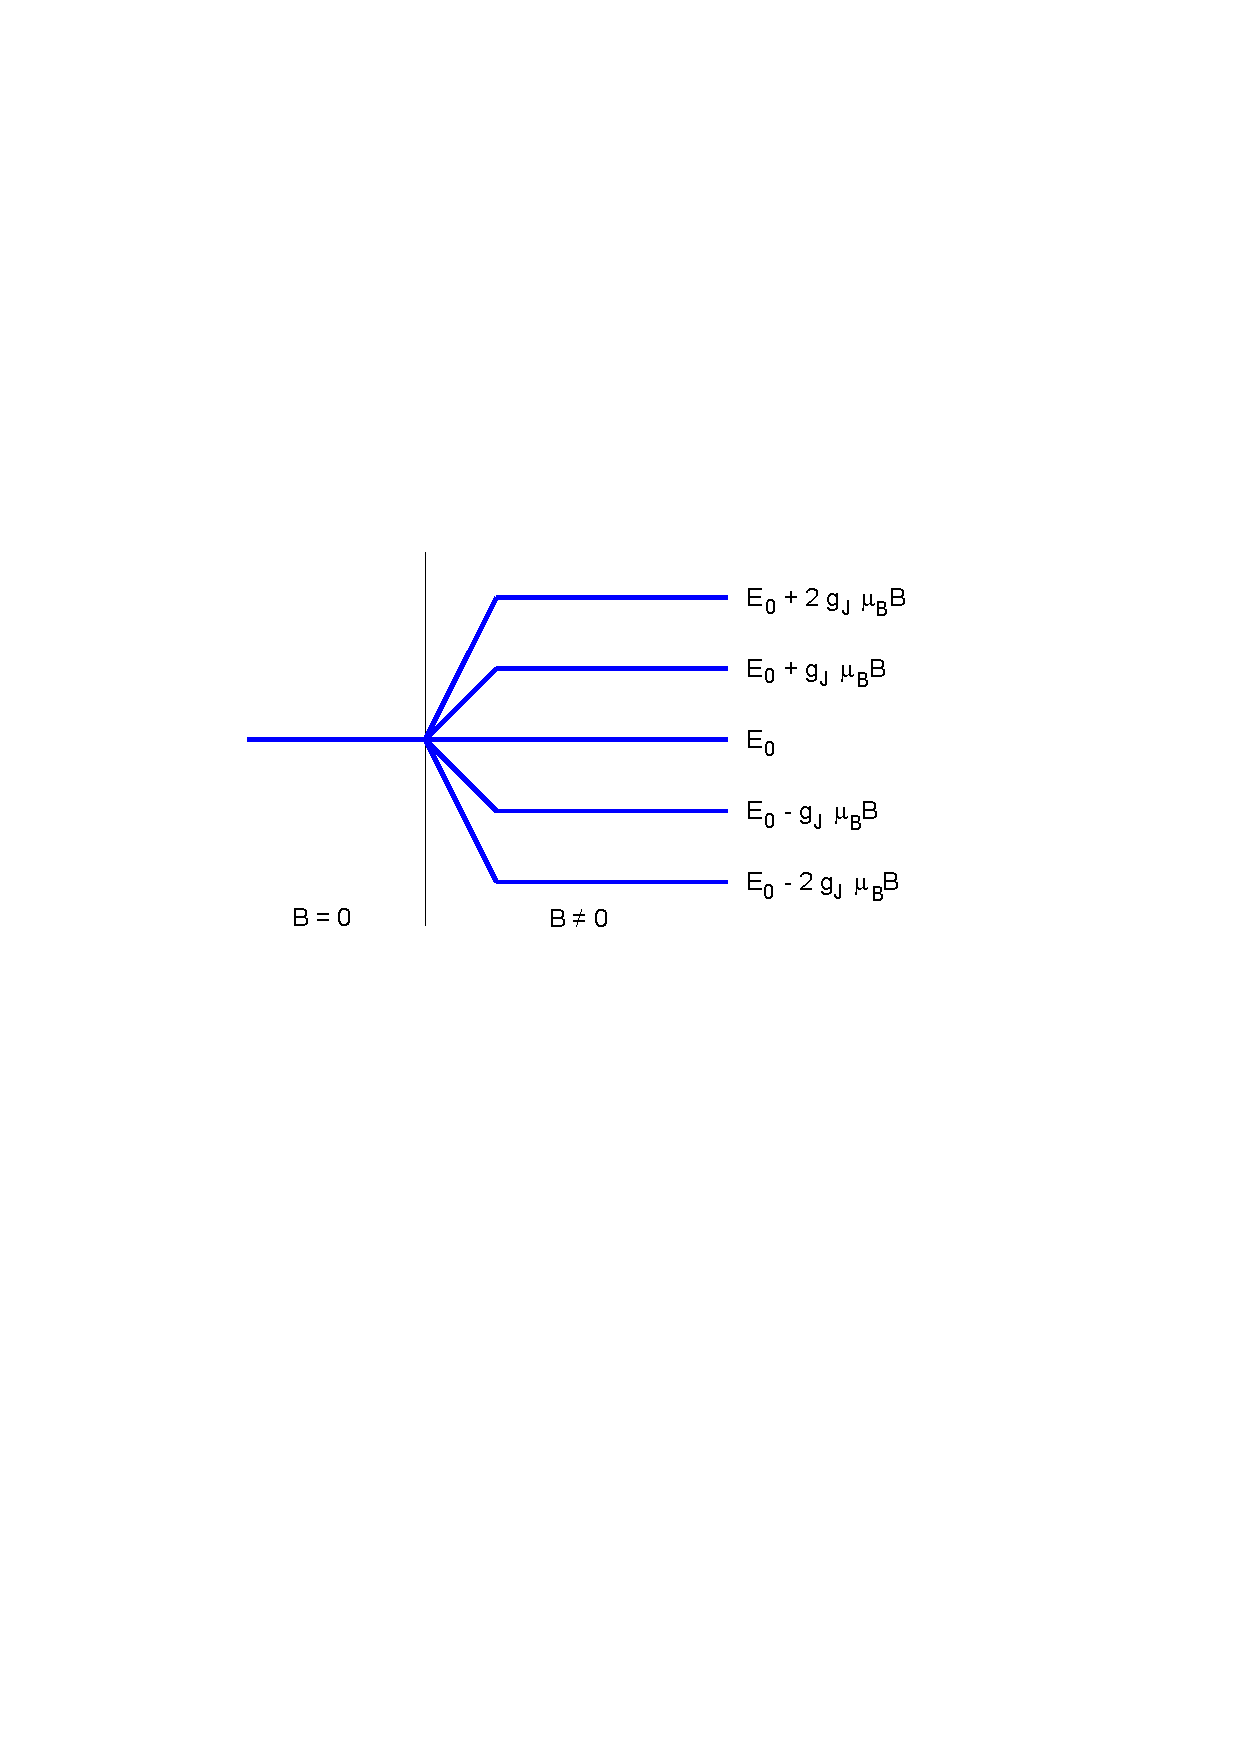
\includegraphics[width=0.6\textwidth]{aufspaltung.pdf}
    \caption{Schematische Darstellung der Aufspaltung eines Energieniveaus eines Atoms mit Gesamtdrehimpulsquantenzahl $J=2$.\cite{anleitung}}
    \label{fig:aufspaltung}
\end{figure}
%
\subsection{Der Zeeman-Effekt}
%
Da in der zeitabhängigen Schrödingergleichung der Spin nicht berücksichtigt wird,
sind die bisherigen Ergebnisse nur für den Fall $S = 0$ gültig. Dies nennt man
den Normalen Zeeman-Effekt. In diesem Fall gilt für
alle $J$, dass $g_J = 1$ ist. Folglich sind die Aufspaltungen unabhängig von den
Quantenzahlen.
\begin{figure}
  \centering
  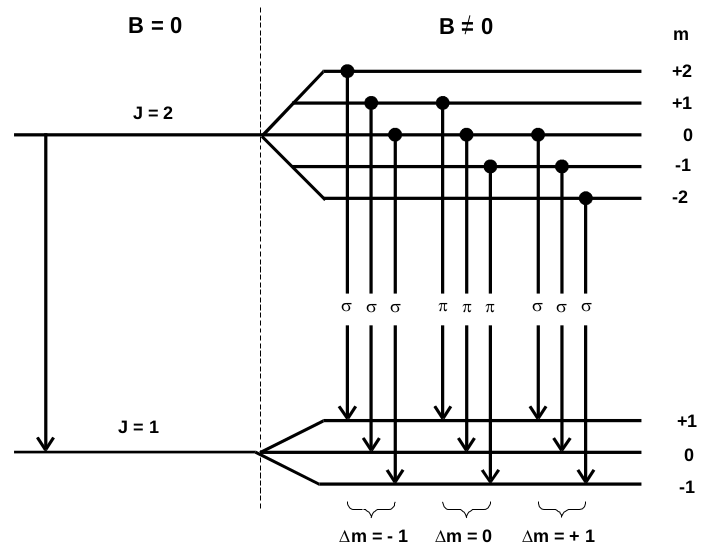
\includegraphics[scale=0.4]{normal.png}
  \caption{Aufspaltung der Energieniveaus und zugehörige Polarisation für den
  normalen Zeeman-Effekt. \cite{anleitung}}
  \label{fig:1}
\end{figure}
Ein Beispiel für eine solche Aufspaltung ist in Abbildung \ref{fig:1} zu sehen.
Dabei ist zu sehen, dass die Energieniveaus äquidistant sind. Es ergibt sich
\begin{equation}
  E_{\symup{mag}}= m \, \mu_B \, B \, .
  \label{eqn:10}
\end{equation}
Die Aufspaltungslinien lassen sich den Auswahlregeln zuordnen, was auch in
Abbildung \ref{fig:1} dargestellt ist. Allerdings sind je nach Beobachtungsrichtung
wegen der unterschiedlichen Polarisation nicht alle Linien zu sehen. Die $\pi$-Linie
(zu $\symup \Delta m = 0$) ist nur sichtbar, wenn die Beobachtungsrichtung
senkrecht zur Feldrichtung, also transversal, ist. Außerdem ist sie gegenüber
der feldfreien Linie nicht verschoben, im Gegensatz zu den Linien mit $\symup \Delta m = \pm 1$,
da sich die Energie um $\mu_B \, B$ im Vergleich zum feldfreien Fall unterscheidet.
Weil sie zirkular polarisiert sind, erscheinen sie bei transversaler Beobachtung als
linear polarisiert.
Der andere Fall, also $S \neq 0$, wird Anomaler Zeeman-Effekt genannt.
Die Auswahlregeln sind auch in diesem Fall noch gültig. Dies lässt
sich über die spinabhängige Schrödingergleichung zeigen. Die Auspaltung wird
vielfältiger, da $g$ nicht mehr für alle $J=1$ ist, sondern von $L, S$ und $J$
abhängt.
\section{Durchführung}
\subsection{Versuchsaufbau}
\begin{figure}
  \centering
  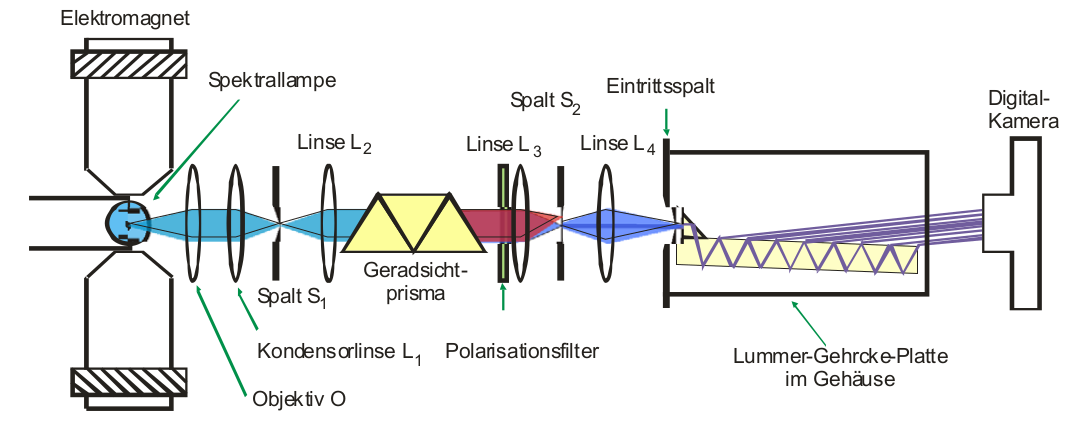
\includegraphics[scale=0.39]{aufbau.png}
  \caption{Der verwendendete Versuchsaufbau. \cite{anleitung}}
  \label{fig:3}
\end{figure}
\noindent
Abbildung \ref{fig:3} zeigt den verwendeten Versuchsaufbau. Das Licht der
verwendeten Cd-Lampe wird in rote und blaue Linien aufgespaltet. Dafür wird die
Lampe in einen starken Elektromagnet gestellt. Dann
wird transversal zum Magnetfeld das Licht nach Wellenlängen aufgespalten. Dies
geschieht durch Linsen, Spalte und ein Geradsichtprisma. Nun kann durch einen
Spalt und einen Polarisationsfilter die gewünschte Linie mit der gewünschten
Polarisation ausgewählt und auf eine Lummer-Gehrke-Platte abgebildet werden.
Dadurch entsteht ein Interferenzmuster. Dieses wird über eine Digitalkamera
aufgenommen. Bei monochromatischem Licht erzeugt die Lummer-Gehrke-Platte
Gangunterschiede von $\lambda$, was die eingestrahlte Wellenlänge ist. Beim
Einschalten des Magnetfeldes tritt eine Verschiebung der Wellenlänge um
$\symup{\Delta} \lambda$ auf, welche wiederum die interferierten Strahlen
um $\symup{\Delta} s$ verschiebt. Dabei wird das Dispersionsgebiet
\begin{equation}
    \symup \symup{\Delta} \lambda_D = \frac{\lambda^2}{2\, d} \cdot \sqrt{\frac{1}{n^2 - 1}}
    \label{eqn:11}
\end{equation}
nicht überschritten, da sonst eine Überlagerung der Wellenlängen auftreten würde.
Hierbei ist $d$ die Dicke der Platte und $n$ die Ordnung des Maximums. Das
Auflösungsvermögen $A$ der Lummer-Gehrke-Platte lässt sich beschreiben durch:
\begin{equation}
  A = \frac{L}{\lambda} (n^2 - 1).
  \label{eqn:12}
\end{equation}
Dabei entspricht $L$ der Länge der Platte und $n$ dem Brechungsindex.
\clearpage
\subsection{Versuchsdurchführung}
Als erstes wird der Elektromagnet, indem das B-Feld über ein Gaußmeter
in Abhängigkeit von dem Feldstrom gemessen wird in einem Intervall von
$0 \leq I \leq \SI{20}{\ampere}$ geeicht.
Daraufhin wird der Aufbau so justiert, dass die gesuchten Wellenlängen
($\lambda = \SI{480}{\nano\meter}$ und $\lambda = \SI{643.8}{\nano\meter}$)
mit der durch den Polarisationsfilter eingestellten Polarisation auf die
Lummer-Gehrke-Platte fallen. Daraufhin wird eine Digitalkamera genutzt, um
Bilder von Interferenzbildern bei verschiedenen Polarisationen und Magnetfeldstärken
aufzunehmen. Dadurch ergibt sich die Wellenlängenverschiebung.

\clearpage
\section{Auswertung}
\label{sec:auswertung}
\subsection{Fehlerrechnung}
Für die Fehlerrechnung sowie den mathematischen Teil der Auswertung wird auf
$\textsc{Python}$ zurückgegriffen:\\
Regressionen sowie deren Fehler wurden durch die $\textsc{Numpy}$ \cite{numpy} Funktion
$\textsc{curve-fit}$ durchgeführt. Grafiken wurden mit $\textsc{Matplotlib}$ \cite{matplotlib}
erstellt.
Fehlerfortpflanzung wird durch die Bibliothek
$\textsc{Uncertainties}$ \cite{uncertainties} automatisiert.

\subsection{"Eichung" des Magnetfeldes}
Um für die weiteren Messungen ein Maß für die stärke des Magnetfeldes bei der Lampe
zu erhalten, wird in einer ersten Messreihe diese in Abhängigkeit von der angelegten
Stromstärke aufgenommen.
Die Ergebnisse dazu stehen in Tabelle \ref{tab:eichung}.
\begin{table}[H]
  \centering
  \caption{Die gemessenen Magnetfeldstärken bei der Lampe mit dem jeweils eingestellten Strom.}
  \label{tab:eichung}
  \begin{tabular}{c c}
    \toprule
    B in \si{\milli\tesla} & I in $\si{\ampere}$ \\
    \midrule
    62  & 1 \\
    120 & 2 \\
    178 & 3 \\
    235 & 4 \\
    290 & 5 \\
    356 & 6 \\
    410 & 7 \\
    462 & 8 \\
    518 & 9 \\
    572 & 10 \\
    625 & 11 \\
    675 & 12 \\
    730 & 13 \\
    780 & 14 \\
    828 & 15 \\
    860 & 16 \\
    890 & 17 \\
    942 & 18 \\
    990 & 19 \\
    \bottomrule
  \end{tabular}
\end{table}
\clearpage
\noindent
Anschließend werden diese Werte linear gefittet.
Für die Steigung $m$ der Geraden und den Y-Achsenabschnitt $b$ ergeben sich:
\begin{align*}
  m &= \SI{51.8(8)}{\milli\tesla\per\ampere}\\
  b &= \SI{36(9)}{\milli\tesla}
\end{align*}
Der entsprechende Graph ist in Abbildung \ref{fig:eichkurve} dargestellt.
\begin{figure}
  \centering
  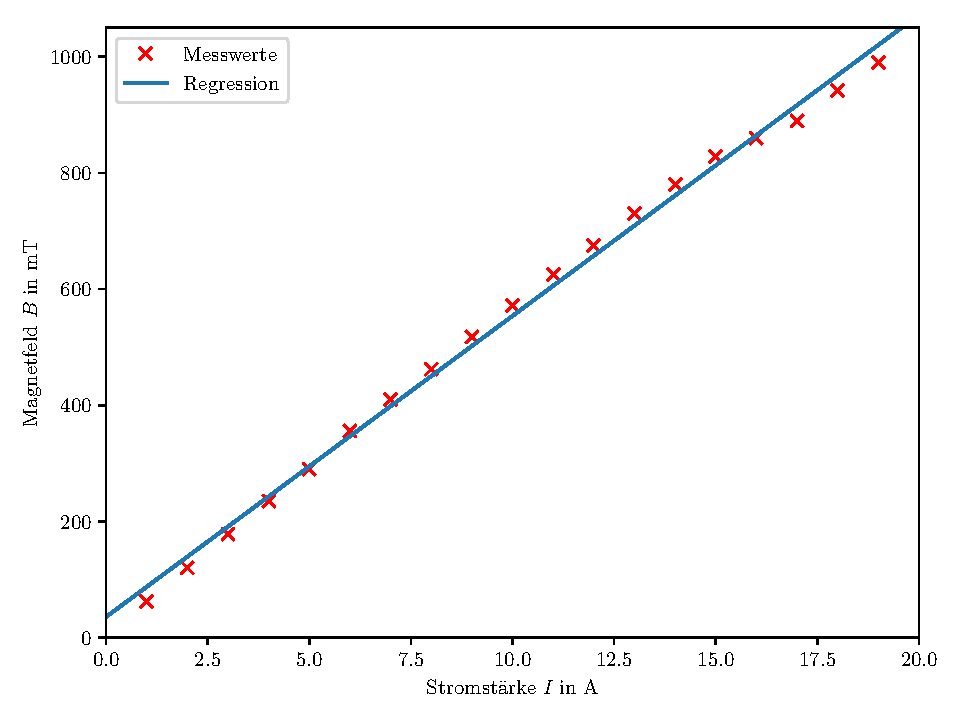
\includegraphics[width=\textwidth]{plot.pdf}
  \caption{Messwerte mit Fit.}
  \label{fig:eichkurve}
\end{figure}\\
Bei den weiteren Messungen wird nun immer die Stromstärke abgelesen und dann mit der
Funktion die entsprechende Magnetfeldstärke bestimmt.
\clearpage
\subsection{Bestimmung der $g_J$ aus der größe der Aufspaltung}
Bei dem Versuch werden zwei Linien des Spektrums einer Cadmiumlampe beobachtet.
Die rote bei $\SI{643.8}{\nano\meter}$ und die blaue bei $\SI{480}{\nano\meter}$.

\noindent
Die rote Linie entsteht bei Übergängen zwischen dem $^1D_2$-Niveau und dem $^1P_1$-Niveau.
Da hier die Multiplizität $M$ für beide Niveaus 1 ist, gilt $S=0$ und somit findet ein
normaler Zeeman-Effekt statt. $g_J$ ist für die bei diesem Übergang beteiligten Niveaus also 1.

\noindent
Die blaue Linie entsteht bei Übergängen zwischen dem $^3P_1$-Niveau und dem $^3S_1$-Niveau.
Aus der Multiplizität ergibt sich für beide Niveaus ein Gesamtspin von 1.
Für das $^3P_1$-Niveau ergibt sich nach Formel \eqref{eq:g_J}
\begin{equation*}
  g_J = \frac{3}{2}
\end{equation*}
und für das $^3S_1$-Niveau ergibt sich
\begin{equation*}
  g_J = 2.
\end{equation*}
Die Größe der Aufspaltung beträgt bei dem anomalen Zeeman-Effekt
\begin{equation}
  \Delta E = g_J \cdot m \mu_B  B.
\end{equation}
Basierend auf diesen Aufspaltungen kommt es nun zu sechs Übergängen zwischen den beiden
Niveaus, welche alle eine unterschiedliche Energie besitzen.
Sie unterscheiden sich um $\pm 2 \mu_B B$, $\pm \frac{3}{2} \mu_B B$ oder $\pm \frac{1}{2} \mu_B B$
von der ursprünglichen Energie der blauen Linie.
Wegen $\Delta m = 0$ ist das Licht, welches die Energie $\Delta E_0 \pm \frac{1}{2} \mu_B B$ besitzt, $\pi$ polarisiert.\\

\noindent
In der Vorbereitung wurde für die verwendete Lummer-Gehrcke-Platte das Dispersionsgebiet $\Delta\lambda_D$
und das Auflösungsvermögen bei einer Wellenlänge von $\SI{643.8}{\nano\meter}$ und
$\SI{480}{\nano\meter}$ berechnet. Das Dispersionsgebiet gibt an wie groß eine Abweichung
der Wellenlänge maximal sein darf, bis sich die entsprechende Linie mit der nächsten Linie überlagert.
Die berechneten Werte sind:
\begin{align*}
  \Delta\lambda_{D_{rot}} &= \SI{4.89e-11}{\meter} \\
  \Delta\lambda_{D_{blau}} &= \SI{2.7e-11}{\meter} \\
  A_{rot} &= 209129 \\
  A_{blau} &= 285458
\end{align*}
Bei abgeschaltetem Magnetfeld entspricht also der Abstand zwischen zwei Maxima einer
Wellenlängendifferenz von $\Delta\lambda_D$. Nun wird zuerst der Abstand $\Delta s$ zwischen
zwei Maxima bei abgeschaltetem Magnetfeld und anschließend die Größe
der Aufspaltung $\delta s$ bei aktivem Magnetfeld gemessen.
Bei der roten Linie lässt sich die größe der Aufspaltung relativ gut messen.
Bei der blauen Linie sind die ausgedruckten Bilder jedoch sehr unscharf. Daher
wird ein Zeichenprogram verwendet um die am Bildschirm deutlich besser zu erkennenden
Maxima mit einer kontrastreicheren Farbe zu markieren und anschließend auf dem Ausdruck
diese Markierungen zu vermessen.
\clearpage
\noindent
Die Bilder befinden sich im Anhang und die gemessenen Werte stehen zusammen mit den eingestellten
B-Feldern in den Tabellen \ref{tab:aufspaltungswerte1} und \ref{tab:aufspaltungswerte2}.
Die Maxima werden dabei entsprechend durchnummeriert.
\begin{table}[H]
  \centering
  \caption{Messwerte von der roten Linie (Bilder 1 und 2).\\ $\delta s$ bei $I=\SI{11.25}{\ampere}\stackrel{\wedge}{=}B=\SI{619(13)}{\milli\tesla}$.}
  \label{tab:aufspaltungswerte1}
  \begin{tabular}{c c c}
    \toprule
    Maximum Nr. & $\Delta s$ in $\si{\centi\meter}$ & $\delta s$ in $\si{\centi\meter}$ \\
    \midrule
     1 & 0.7  & 0.35 \\
     2 & 0.8  & 0.35 \\
     3 & 0.85 & 0.4  \\
     4 & 0.9  & 0.4  \\
     5 & 1    & 0.5  \\
     6 & 1.05 & 0.5  \\
     7 & 1.2  & 0.6  \\
     8 & 1.4  & 0.7  \\
     9 & 1.7  & 0.75 \\
    \bottomrule
  \end{tabular}
\end{table}
\noindent
Die Ströme zu den Magnetfeldern, die bei der blauen Linie eingestellt wurden stehen
in Tabelle \ref{tab:ströme}.
\begin{table}[H]
  \centering
  \caption{Die Stromstärken zu den $B$ Feldern in Tabelle \ref{tab:aufspaltungswerte2}.}
  \label{tab:ströme}
  \begin{tabular}{c c}
    \toprule
    $I$ in $\si{\ampere}$ & $B$ in $\si{\milli\tesla}$ \\
    \midrule
    9.75  & $\SI{541(12)}{}$  \\
    13.4  & $\SI{730(14)}{}$  \\
    15.25 & $\SI{826(15)}{}$  \\
    16    & $\SI{865(16)}{}$  \\
    19.4  & $\SI{1041(18)}{}$ \\
    \bottomrule
  \end{tabular}
\end{table}

\noindent
Da bei der Zeemanaufspaltung eine Wellenlängenaufspaltung in beide Richtungen stattfindet
(größer und kleiner als die ursprüngliche Wellenlänge) entspricht $\delta s$ der zweifachen
Wellenlängendifferenz $\delta\lambda$.
Damit lässt sich die Wellenlängendifferenz der Aufspaltung berechnen nach:
\begin{equation}
  \delta\lambda = \frac{1}{2} \frac{\delta s}{\Delta s} \Delta\lambda_D
\end{equation}
Die einzelnen Wellenlängendifferenzen stehen in Tabelle \ref{tab:wellenl} und die Mittelwerte in Tabelle \ref{tab:wellenl2}.
Die Mittelwerte werden dabei immer über die Differenzen gebildet, die bei der gleichen
Magnetfeldstärke aufgenommen wurden.
\clearpage
\begin{landscape}
  \begin{table}[H]
    \centering
    \caption{Messwerte von der blauen Linie. Bei Bild 4 ist $\Delta s$ angegeben. Für die Anderen $\delta s$. Der Index steht für die Nr. des Maximums.}
    \label{tab:aufspaltungswerte2}
    \begin{tabular}{c c c c c c c c c}
      \toprule
      Bild Nr. & $\Delta s_1$ | $\delta s_1$ & $\Delta s_2$ | $\delta s_2$ & $\Delta s_3$ | $\delta s_3$ & $\Delta s_4$ | $\delta s_4$ & $\Delta s_5$ | $\delta s_5$ & $\Delta s_6$ | $\delta s_6$ & $B$ in $\si{\milli\tesla}$ & Polarisierung \\
      \midrule
       4 & $\SI{0.75}{\centi\meter}$ & $\SI{0.8 }{\centi\meter}$ & $\SI{0.9 }{\centi\meter}$ & $\SI{1   }{\centi\meter}$ & $\SI{1.15}{\centi\meter}$ & $\SI{1.25}{\centi\meter}$ & $\SI{0}{}$ & $\sigma$ \\
       5 & $\SI{0.2 }{\centi\meter}$ & $\SI{0.2 }{\centi\meter}$ & $\SI{0.25}{\centi\meter}$ & $\SI{0.3 }{\centi\meter}$ & $\SI{0.3 }{\centi\meter}$ & $\SI{0.4 }{\centi\meter}$ & $\SI{541(12)}{}$ & $\sigma$ \\
       6 & $\SI{0.25}{\centi\meter}$ & $\SI{0.35}{\centi\meter}$ & $\SI{0.3 }{\centi\meter}$ & $\SI{0.3 }{\centi\meter}$ & $\SI{0.35}{\centi\meter}$ & $\SI{0.4 }{\centi\meter}$ & $\SI{730(14)}{}$ & $\sigma$ \\
       7 & $\SI{0.2 }{\centi\meter}$ & $\SI{0.3 }{\centi\meter}$ & $\SI{0.35}{\centi\meter}$ & $\SI{0.35}{\centi\meter}$ & $\SI{0.4 }{\centi\meter}$ & $\SI{0.4 }{\centi\meter}$ & $\SI{826(15)}{}$ & $\sigma$ \\
       9 & $\SI{0.25}{\centi\meter}$ & $\SI{0.3 }{\centi\meter}$ & $\SI{0.3 }{\centi\meter}$ & $\SI{0.35}{\centi\meter}$ & $\SI{0.4 }{\centi\meter}$ & $\SI{0.45}{\centi\meter}$ & $\SI{826(15)}{}$ & $\sigma$ \\
      10 & $\SI{0.3 }{\centi\meter}$ & $\SI{0.3 }{\centi\meter}$ & $\SI{0.35}{\centi\meter}$ & $\SI{0.4 }{\centi\meter}$ & $\SI{0.4 }{\centi\meter}$ & $\SI{0.45}{\centi\meter}$ & $\SI{865(16)}{}$ & $\sigma$ \\
      12 & $\SI{0.2 }{\centi\meter}$ & $\SI{0.25}{\centi\meter}$ & - & - & - & - & $\SI{1041(18)}{}$ & $\pi$ \\
      \bottomrule
    \end{tabular}
  \end{table}
\end{landscape}
\begin{landscape}
\begin{table}[H]
  \centering
  \caption{Wellenlängendifferenzen $\delta \lambda$.}
  \label{tab:wellenl}
  \begin{tabular}{c c c c c c c c}
    \toprule
    Bild: 2 & 5 & 6 & 7 & 9 & 10 & 12 \\
    \midrule
    $\SI{1.22e-11}{\meter}$ & $\SI{3.60e-12}{\meter}$ & $\SI{4.50e-12}{\meter}$ & $\SI{3.60e-12}{\meter}$ & $\SI{4.50e-12}{\meter}$ & $\SI{5.40e-12}{\meter}$ & $\SI{5.40e-12}{\meter}$ \\
    $\SI{1.07e-11}{\meter}$ & $\SI{3.38e-12}{\meter}$ & $\SI{5.91e-12}{\meter}$ & $\SI{5.06e-12}{\meter}$ & $\SI{5.06e-12}{\meter}$ & $\SI{5.06e-12}{\meter}$ & $\SI{5.91e-12}{\meter}$ \\
    $\SI{1.15e-11}{\meter}$ & $\SI{3.75e-12}{\meter}$ & $\SI{4.50e-12}{\meter}$ & $\SI{5.25e-12}{\meter}$ & $\SI{4.50e-12}{\meter}$ & $\SI{5.25e-12}{\meter}$ &  \\
    $\SI{1.09e-11}{\meter}$ & $\SI{4.05e-12}{\meter}$ & $\SI{4.05e-12}{\meter}$ & $\SI{4.73e-12}{\meter}$ & $\SI{4.73e-12}{\meter}$ & $\SI{5.40e-12}{\meter}$ &  \\
    $\SI{1.22e-11}{\meter}$ & $\SI{3.52e-12}{\meter}$ & $\SI{4.11e-12}{\meter}$ & $\SI{4.70e-12}{\meter}$ & $\SI{4.70e-12}{\meter}$ & $\SI{4.70e-12}{\meter}$ &  \\
    $\SI{1.16e-11}{\meter}$ & $\SI{4.32e-12}{\meter}$ & $\SI{4.32e-12}{\meter}$ & $\SI{4.32e-12}{\meter}$ & $\SI{4.86e-12}{\meter}$ & $\SI{4.86e-12}{\meter}$ &  \\
    $\SI{1.22e-11}{\meter}$ &  &  &  &  &  &  \\
    $\SI{1.22e-11}{\meter}$ &  &  &  &  &  &  \\
    $\SI{1.08e-11}{\meter}$ &  &  &  &  &  &  \\
    \bottomrule
  \end{tabular}
\end{table}
\begin{table}[H]
  \centering
  \caption{Mittelwerte von $\delta \lambda$.}
  \label{tab:wellenl2}
  \begin{tabular}{c c}
    \toprule
    Bild: & Mittelwert $\delta\lambda$ \\
    \midrule
    2 & $\SI{1.16(2)e-11}{\meter}$ \\
    5 & $\SI{3.77(1)e-12}{\meter}$ \\
    6 & $\SI{4.56(3)e-12}{\meter}$ \\
    7u.9 & $\SI{4.67(1)e-12}{\meter}$ \\
    10 & $\SI{5.11(1)e-12}{\meter}$ \\
    12 & $\SI{5.65(3)e-12}{\meter}$ \\
    \bottomrule
  \end{tabular}
\end{table}
\end{landscape}
\noindent
Zuletzt wird die Wellenlängendifferenz in die Energiedifferenz und
diese über die Magnetfeldstärke in $g_J$ umgerechnet:
\begin{align}
  \Delta E &= \frac{h \cdot c}{\lambda_0}-\frac{h \cdot c}{\lambda_0+\delta\lambda}\\
  \Delta E &= g_J \cdot \mu_B B\\
  => g_J &= \left(\frac{h \cdot c}{\lambda_0}-\frac{h \cdot c}{\lambda_0+\delta\lambda}\right) / \mu_B B
\end{align}
$\lambda_0$ ist dabei die Wellenlänge der Linie ohne Magnetfeld. $h$ ist die Planck-Konstante, $c$ die Lichtgeschwindigkeit
und $\mu_B$ das bohrsche Magneton. Für diese Konstanten werden immer die Werte von Scipy \cite{scipy} verwendet.
Damit ergeben sich dann die Werte für $g_J$, welche in Tabelle \ref{tab:gjergebnisse} stehen.
Die Theoriewerte sind dort ebenfalls aufgelistet.
\begin{table}[H]
  \centering
  \caption{Die berechneten Werte von $g_J$ und die Theoriewerte}
  \label{tab:gjergebnisse}
  \begin{tabular}{c c c}
    \toprule
    Bild: & $g_J$ & Theorie \\
    \midrule
    2 & $\SI{0.969(27)}{}$ & 1 \\
    5 & $\SI{0.648(29)}{}$ & 2 oder 1.5 \\
    6 & $\SI{0.58(4)}{}$ & 2 oder 1.5 \\
    7 u. 9 & $\SI{0.525(17)}{}$ & 2 oder 1.5 \\
    10 & $\SI{0.549(16)}{}$ & 2 oder 1.5 \\
    12 & $\SI{0.505(24)}{}$ & 0.5 \\
    \bottomrule
  \end{tabular}
\end{table}
\section{Diskussion}
Beim Betrachten der Ergebnisse fällt sofort auf, dass die Werte bei der roten Linie
und bei dem $\pi$ Übergang, welcher auf Bild 12 zu sehen ist, sehr nah an die Theoriewerte heran kommen.
Die Werte für die $\sigma$ Übergänge der blauen Linie liegen allerdings deutlich unter den Theoriewerten.
Mögliche Gründe dafür sind die generell etwas unscharfen Aufnahmen der blauen Aufspaltungen und eventuell
auch eine Fehlinterpretation der Bilder. Bei den Polarisationswinkeln scheint etwas durcheinander gekommen zu sein.
demnach könnte es durchaus sein, dass die Bilder 5, 6, 7, 9 und 10 eigentlich die $\pi$ Aufspaltung zeigen und Bild 12 die
$\sigma$ Aufspaltung. Bei dem entsprechenden Magnetfeld von Bild 12 wäre die Aufspaltung theoretisch so groß, dass sich die Maxima überlagern
könnten. Bei der Aufzeichnung der Bilder wurden die Polarisationswinkel notiert. Allerdings schien für uns die Aufspaltung in den Bildern 5, 6, 7, 9 und 10
die $\sigma$ Aufspaltung zu sein. Auf Bild 8 ist die gleiche Polarisationsrichtung abgebildet, wie auf Bild 12.
Die Aufspaltung ist dort fast nicht zu erkennen. Das Magnetfeld sollte allerdings mit $\SI{826(15)}{\milli\tesla}$ klein genug sein,
damit auf diesem Bild, sofern es die $\sigma$ Aufspaltung zeigen würde, eine Aufspaltung deutlich zu erkennen sein müsste
und die Maxima sich dabei noch nicht überlagern.
Wenn die angenommenen Polarisationswinkel stimmen scheint die Aufspaltung durch andere Gründe wesentlich kleiner auszufallen
als sie es eigentlich tun sollte.
\newpage
\nocite{*}
\printbibliography

\end{document}
